%===================================================================================
\chapter{Code Organization}\label{s:organization}
%===================================================================================

%----------------------------------
\section{SUNDIALS organization}\label{ss:sun_org}
%----------------------------------
% This is a shared SUNDIALS TEX file with description of
% the SUNDIALS organization
%
The family of solvers referred to as {\sundials} consists of the solvers
{\cvode} (for ODE systems), {\kinsol} (for nonlinear algebraic
systems), and {\ida} (for differential-algebraic systems).  In addition,
{\sundials} also includes variants of {\cvode} and {\ida} with sensitivity analysis 
capabilities (using either forward or adjoint methods): {\cvodes} and {\idas},
respectively.

The various solvers of this family share many subordinate modules.
For this reason, it is organized as a family, with a directory
structure that exploits that sharing (see Fig. \ref{f:sunorg}).
\begin{figure}
\subfigure[High-level diagram]
{\centerline{\psfig{figure=sunorg1.eps,width=\textwidth}}}
\subfigure[Directory structure of the source tree]
{\centerline{\psfig{figure=sunorg2.eps,width=\textwidth}}}
\caption {Organization of the SUNDIALS suite}\label{f:sunorg}
\end{figure}
The following is a list of the solver packages presently available:
\begin{itemize}

\item {\cvode},  
  a solver for stiff and nonstiff ODEs $dy/dt = f(t,y)$;

\item {\cvodes},
  a solver for stiff and nonstiff ODEs
  with sensitivity analysis capabilities;

\item {\ida},
  a solver for differential-algebraic systems $F(t,y,y^\prime) = 0$;

\item {\idas},
  a solver for differential-algebraic systems
  with sensitivity analysis capabilities;

\item {\kinsol}, 
  a solver for nonlinear algebraic systems $F(u) = 0$.

\end{itemize}


%----------------------------------
\section{IDA organization}\label{ss:ida_org}
%----------------------------------

\index{IDA@{\ida}!package structure}
The {\ida} package is written in the ANSI {\CC} language. The following
summarizes the basic structure of the package, although knowledge
of this structure is not necessary for its use.

The overall organization of the {\ida} package is shown in Figure
\ref{f:idaorg}.
\begin{figure}
{\centerline{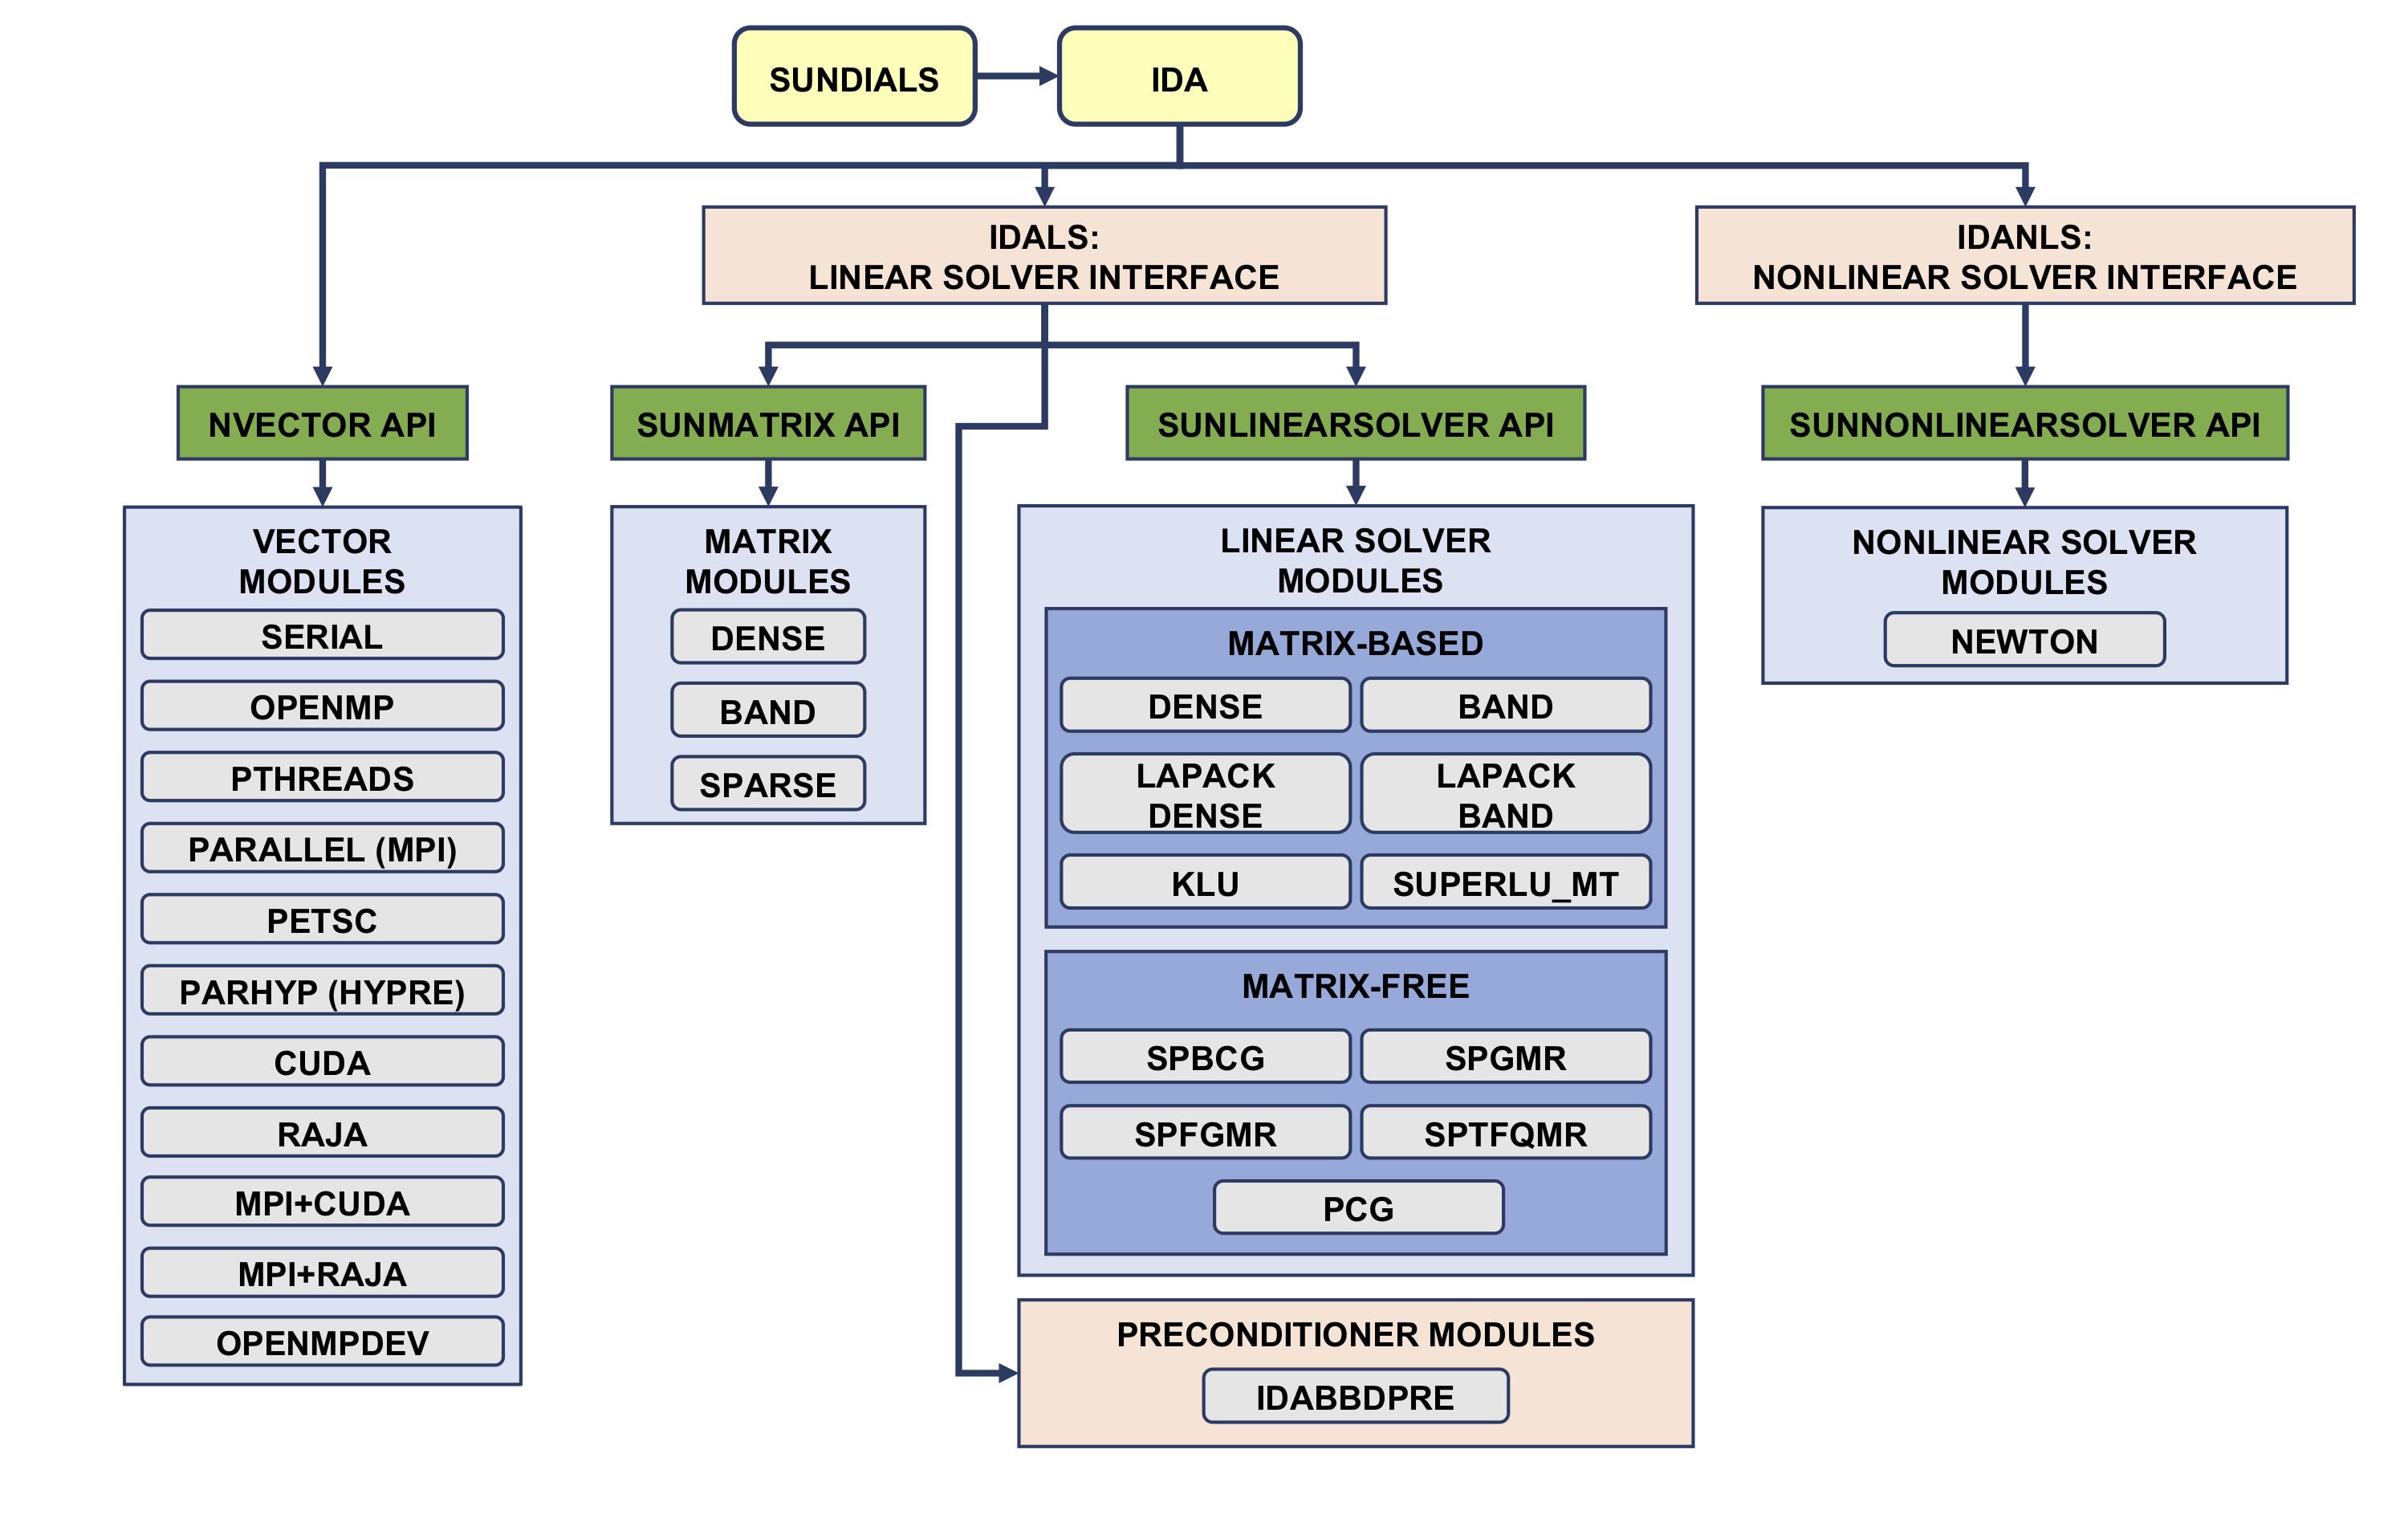
\includegraphics[width=\textwidth]{idaorg}}}
\caption [Overall structure diagram of the {\ida} package]
{Overall structure diagram of the {\ida} package.
  Modules specific to {\ida} begin with ``IDA'' ({\idals},
  {\idabbdpre}, and {\idanls}), all other items correspond
  to generic solver and auxiliary modules. 
  Note also that the LAPACK, {\klu} and {\superlumt} support is
  through interfaces to external packages. 
  Users will need to download and compile those packages independently.}
\label{f:idaorg}
\end{figure}
The central integration module, implemented in the files \id{ida.h},
\id{ida\_impl.h}, and \id{ida.c}, deals with the evaluation of integration 
coefficients, estimation of local error,
selection of stepsize and order, and interpolation to user output
points, among other issues.

{\ida} utilizes generic linear and nonlinear solver modules defined by the
{\sunlinsol} API (see Chapter \ref{s:sunlinsol}) and {\sunnonlinsol} API (see
Chapter \ref{c:sunnonlinsol}) respectively. As such, {\ida} has no knowledge
of the method being used to solve the linear and nonlinear systems that
arise in each time step. For any given user problem, there exists a single
nonlinear solver interface and, if necessary, a linear system solver
interface is specified, and invoked as needed during the integration. While
{\sundials} includes a fixed-point nonlinear solver module, it is not currently
supported in {\ida} (note the fixed-point module is listed in Figure
\ref{f:sunorg1} but not Figure \ref{f:idaorg}).

\index{IDA@{\ida} linear solver interfaces|(} 
{\ida} now has a single unified linear solver interface, {\idals},
supporting both direct and iterative linear solvers built using the
generic {\sunlinsol} API (see Chapter \ref{s:sunlinsol}).  These
solvers may utilize a {\sunmatrix} object (see Chapter
\ref{s:sunmatrix}) for storing Jacobian information, or they may be
matrix-free.  Since {\ida} can operate on any valid {\sunlinsol}
implementation, the set of linear solver modules available to {\ida}
will expand as new {\sunlinsol} modules are developed.

For users employing dense or banded Jacobian matrices, {\idals}
includes algorithms for their approximation through difference 
quotients, but the user also has the option of supplying the Jacobian
(or an approximation to it) directly.  This user-supplied 
routine is required when using sparse or user-supplied Jacobian
matrices.

For users employing matrix-free iterative linear solvers, {\idals}
includes an algorithm for the approximation by difference quotients of
the product between the Jacobian matrix and a vector, $Jv$. Again, the
user has the option of providing routines for this operation, in two
phases: setup (preprocessing of Jacobian data) and multiplication.

For preconditioned iterative methods, \index{preconditioning!setup and solve phases} 
the preconditioning must be supplied by the user, again in two phases: 
setup and solve.  While\index{preconditioning!advice on} there is no
default choice of preconditioner analogous to the difference-quotient
approximation in the direct case, the references
\cite{BrHi:89,Byr:92}, together with the example and demonstration
programs included with {\ida}, offer considerable assistance in
building preconditioners. 

\index{IDA@{\ida} linear solvers!implementation details|(} 
{\ida}'s linear solver interface consists of four primary routines,
devoted to (1) memory allocation and initialization, (2) setup of the
matrix data involved, (3) solution of the system, and (4) freeing of memory.  
The setup and solution phases are separate because the evaluation of
Jacobians and preconditioners is done only periodically during the
integration, as required to achieve convergence. The call list within
the central {\ida} module to each of the four associated functions is
fixed, thus allowing the central module to be completely independent
of the linear system method.
\index{IDA@{\ida} linear solvers!implementation details|)} 

{\ida} also provides a preconditioner module, {\idabbdpre}, for use
with any of the Krylov iterative linear solvers.  It works in
conjunction with {\nvecp} and generates a preconditioner that is a  
block-diagonal matrix with each block being a banded matrix.

All state information used by {\ida} to solve a given problem is saved
in a structure, and a pointer to that structure is returned to the
user.  There is no global data in the {\ida} package, and so, in this
respect, it is reentrant. State information specific to the linear
solver is saved in a separate structure, a pointer to which resides in
the {\ida} memory structure. The reentrancy of {\ida} was motivated
by the situation where two or more problems are solved by
intermixed calls to the package from one user program.
